\subsection{Sistema de Control}

En forma general, el sistema de control es el bloque de la plataforma que se encarga de tomar los datos de las señales medidas por los distintos sensores, convertirlos a una forma utilizable por el sistema, y luego, mediante un análisis de los mismos, generar señales de comando que se envían al convertidor para modificar su comportamiento, buscando llegar a un punto de funcionamiento adecuado para las condiciones existentes.\\

Todas estas tareas son llevadas a cabo por un módulo llamado {\Medium controlador digital de señales} o DSC (del inglés \textit{Digital Signal Controller}). Este dispositivo, como indica su nombre, es un microcontrolador convencional, pero que contiene ciertas modificaciones en su arquitectura de hardware y su repertorio de instrucciones (por ejemplo, hardware dedicado para la operación de \textit{Multiply-and-Accumulate}) que lo adecuan para su uso en el procesamiento de señales digitales.\\

Para esta plataforma, se utiliza un DSC perteneciente a la linea {\Medium C2000} de microcontroladores de tiempo real de Texas Instruments. En particular, se utiliza el modelo {\Medium TMS320F28335} de arquitectura de bus tipo Harvard, con \SI[]{150}{\mega\hertz} de frecuencia de reloj, CPU de 32 bits, memoria flash de 256K palabras de 16 bits, conversor analógico-digital de 12 bits y 16 canales, módulos de comunicación serie SPI, I\textsuperscript{2}C, y UART, entre múltiples otras funcionalidades.\textsuperscript{\cite{DSP-Datasheet}}\\

\begin{figure}[h]
    \centering
    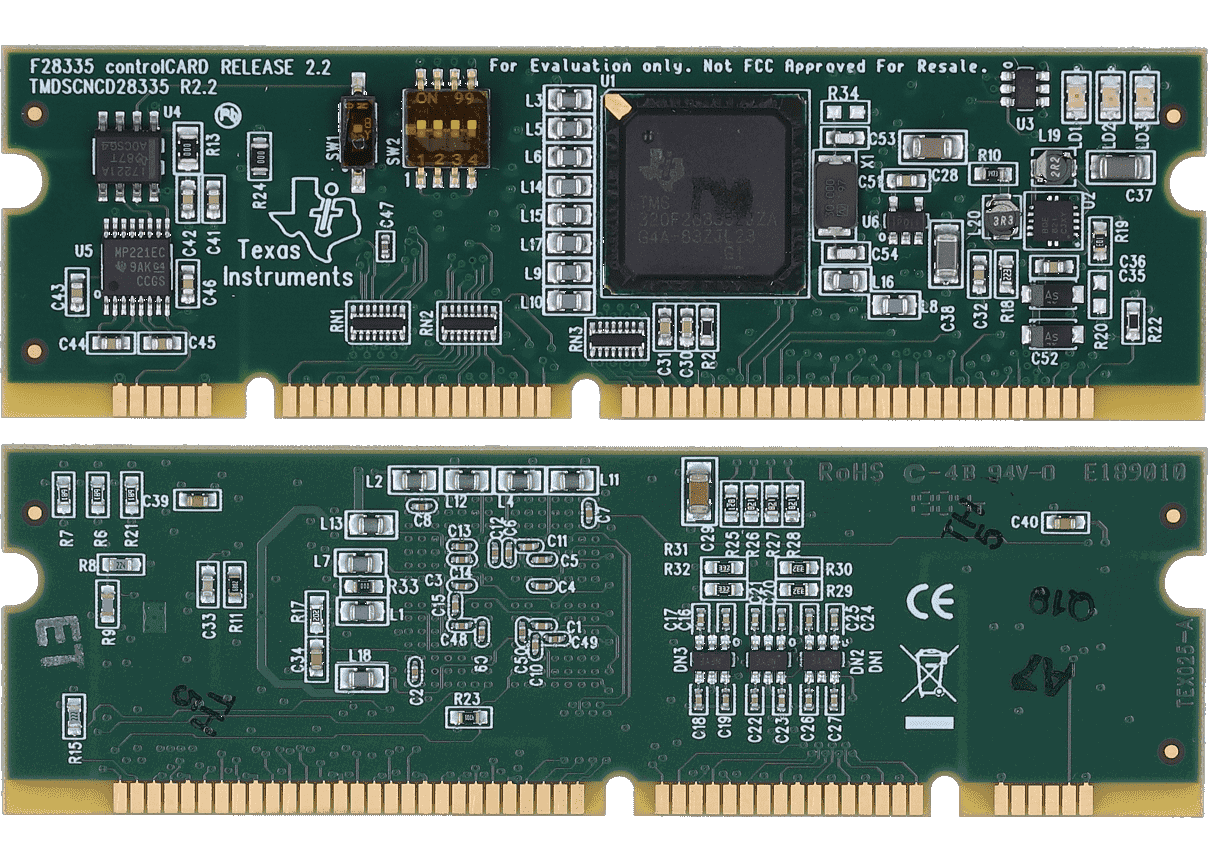
\includegraphics[scale=0.22]{Imagenes/ControlCARD.png}
    \caption{Controlador digital de señales modelo TMS320F28335 de la linea C2000, en su paquete de evaluación tipo ControlCARD, para inserción en slot DIMM-100.}
    \label{ControlCARD}
\end{figure}